\section{Pruebas de requerimientos no funcionales}
Los requerimientos no funcionales mencionados en la sección \ref{RequerimientosNF}, fueron probados de la siguiente manera.

\subsection{RNF1. Escalabilidad}

La arquitectura de microservicios nos permite ejecutar diversas instancias de un mismo servidor aunque se encuentren en otros dispositivos físicos. A continuación se muestra una captura de pantalla que muestra como dos microservicios sirven el mismo servicio.

En la Figura \ref{fig:micro1}, se muestra como existe solamente un microservicio en funcionamiento para cada uno de los servicios.
\begin{figure}[H]
	\centering
	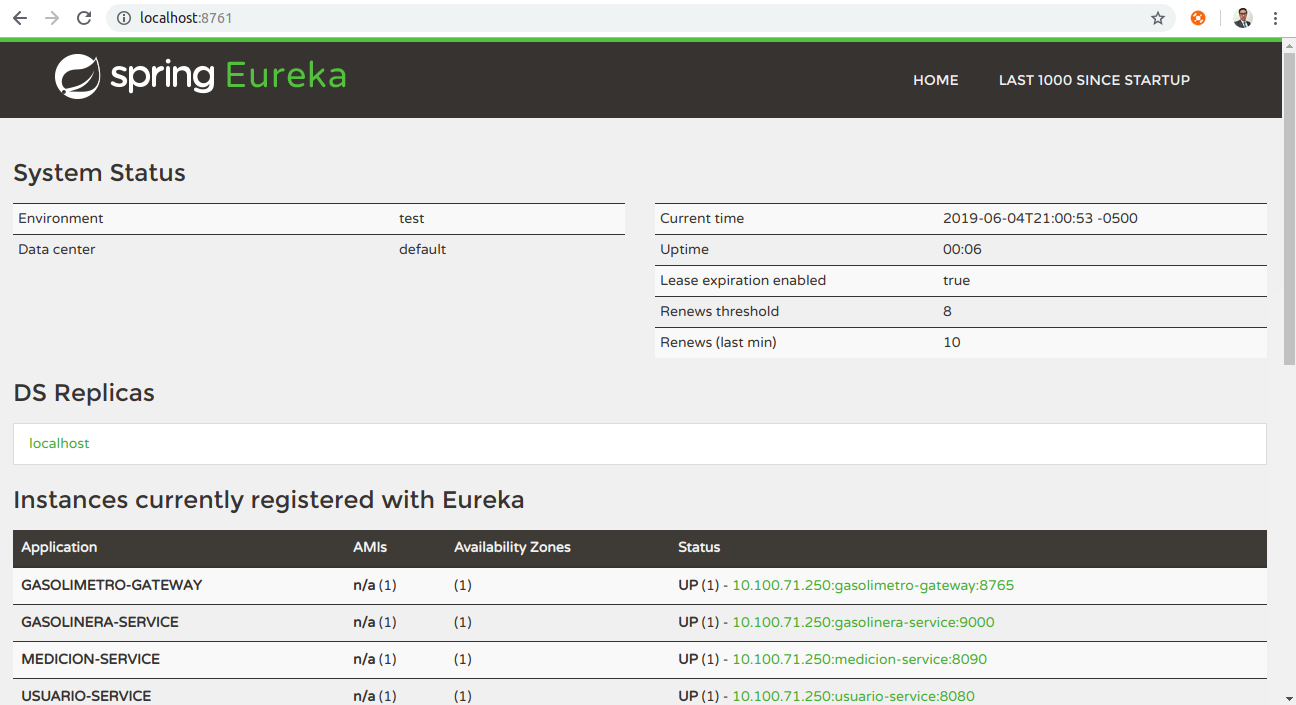
\includegraphics[scale=.36]{Capitulo6/no-funcionales/images/micro1}
	\caption{Captura de pantalla cada servicio con un solo microservicio}
	\label{fig:micro1}
\end{figure}

Posteriormente, se activa otro microservicio para cada servicio, los cuales se pueden observar funcionando en la Figura \ref{fig:micro2}. 

\begin{figure}[H]
	\centering
	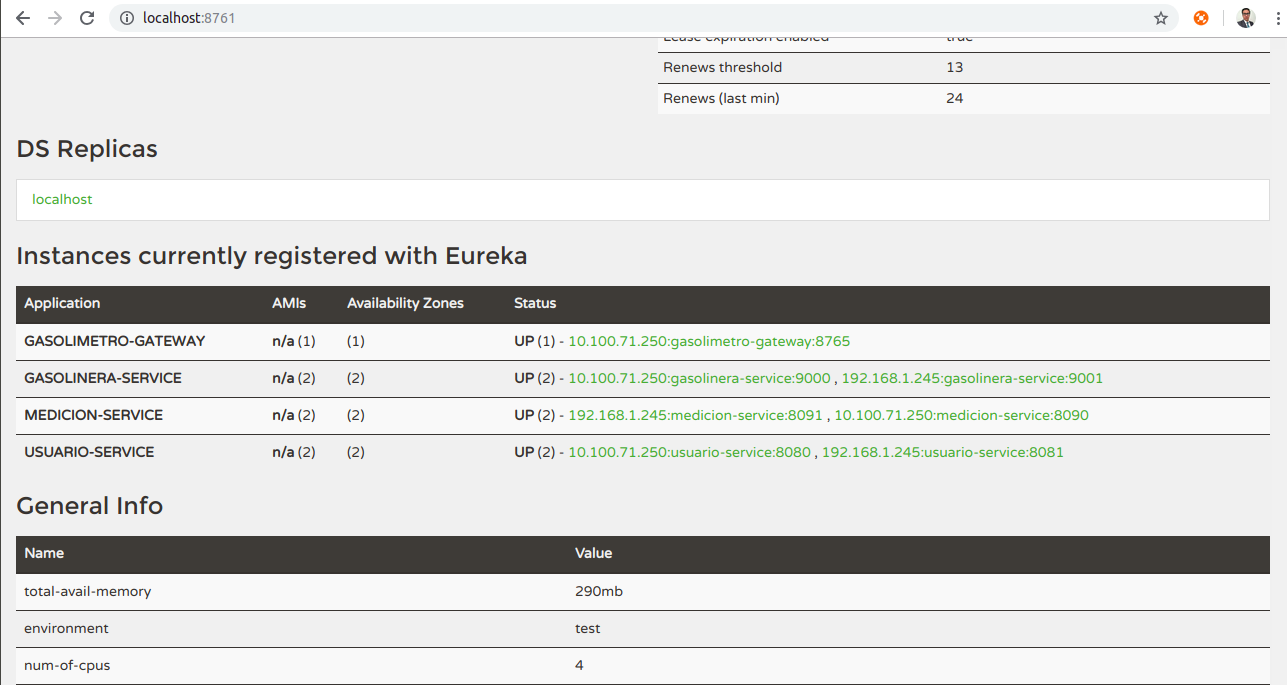
\includegraphics[scale=.36]{Capitulo6/no-funcionales/images/micro2}
	\caption{Captura de pantalla cada servicio con dos microservicios}
	\label{fig:micro2}
\end{figure}


\subsection{RNF2. Seguridad}

En la Figura \ref{fig:verificar}, se muestra un ejemplo de un correo electrónico enviado a un usuario, solicitando que verifique su cuenta.

\begin{figure}[H]
	\centering
	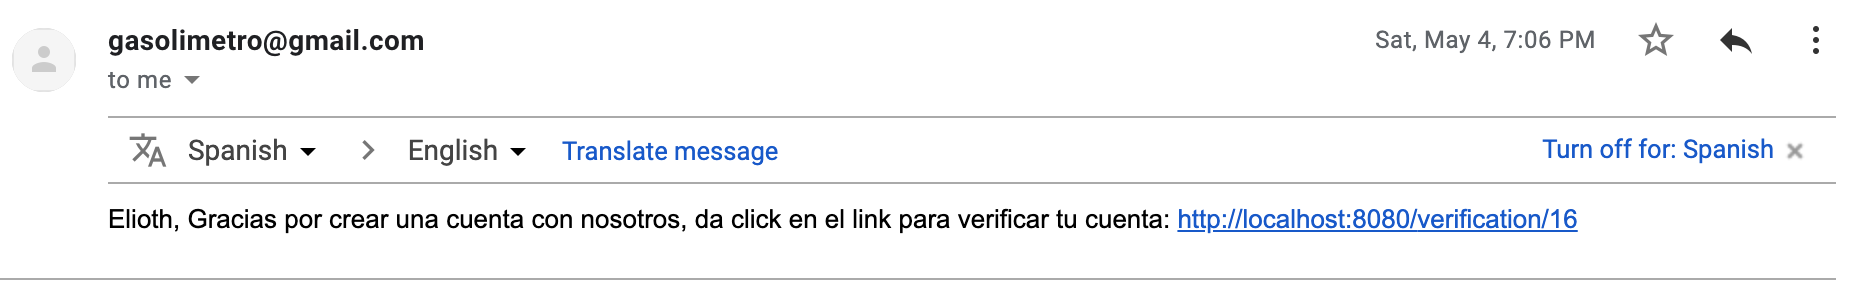
\includegraphics[scale=.45]{Capitulo6/no-funcionales/images/verificar}
	\caption{Captura de pantalla de un correo electrónico de verificación de cuenta enviado}
	\label{fig:verificar}
\end{figure}


\subsection{RNF3. Usabilidad}

Para comprobar este requerimiento no funcional, se trabajo con usuarios potenciales de nuestro mercado objetivo. El cual corresponde a automovilistas de la Ciudad de México. En estas pruebas, se les solicitaba realizar alguna acción dentro de la aplicación y posteriormente era medido el tiempo que al usuario le tomaba realizar la acción, los resultados se muestran en la tabla \ref{pruebas_usabilidad}.
\begin{longtable}{|M{2cm}| M{4.5cm}|M{3cm}|M{3cm}|M{1.5cm}|}
	\hline
	\textbf{No. prueba} & \textbf{Nombre usuario} & \textbf{Acción} & \textbf{Tiempo tardado} & \textbf{Prueba exitosa} \\ \hline
	1 & Samuel Arteaga Lara & Consultar la información de una gasolinera & 15 segundos & Si \\ \hline
	2 & Samuel Arteaga Lara & Registrarse como Cliente & 10 segundos & Si \\ \hline
	3 & Samuel Arteaga Lara & Verificar su cuenta & 30 segundos & Si \\ \hline
	4 & Andrés Saldaña Aguilar & Iniciar sesión con un usuario y contraseña dados & 8 segundos & Si \\ \hline
	5 & Andrés Saldaña Aguilar & Registrar una medición de prueba & 10 segundos & Si \\ \hline
	6 & Andrés Saldaña Aguilar & Agregar un automóvil & 11 segundos & Si \\ \hline
	7 & Andrés Saldaña Aguilar & Agregar un sensor & 6 segundos & Si \\ \hline
	8 & Miguel Garcia Cebada & Obtener la ruta entre la posición actual y alguna gasolinera & 2 segundos & Si \\ \hline
	9 & Miguel Garcia Cebada & Asociar un automóvil con un sensor & 10 segundos & Si \\ \hline
	10 & Miguel Garcia Cebada & Crear un reporte & 12 segundos & Si \\ \hline
	\caption{Resultados de las pruebas sobre usabilidad en la aplicación móvil}
	\label{pruebas_usabilidad}
\end{longtable}


\subsection{RNF4. Tiempo de ejecución}

Para comprobar este requerimiento no funcional, se midió el tiempo de ejecución de los casos de uso que más procesamientos realizan, los resultados obtenidos se muestran en la tabla \ref{pruebas_ejecucion}.
\begin{longtable}{|M{2cm}| M{4.5cm}|M{3cm}|M{3cm}|M{1.5cm}|}
	\hline
	\textbf{No. prueba} & \textbf{Nombre caso de uso} & \textbf{Entrada} & \textbf{Tiempo tardado (en segundos)} & \textbf{Prueba exitosa} \\ \hline
	1 & SUB-C-CU1-Generar clasificación & 10,000 gasolineras & 120 & Si \\ \hline
	2 & SUB-C-CU2-Consultar mapa & 8 gasolineras & 0.4 & Si \\ \hline
	3 & SUB-C-CU2.2-Consultar gasolinera & 1 gasolinera & 0.1 & Si \\ \hline
	4 & SUB-M-CU1.1.1-Almacenar medición & 1 medición con precio y bomba & 0.14 & Si \\ \hline
	5 & SUB-U-CU1-Registrar usuario & 1 usuario & 0.21 & Si \\ \hline
	6 & SUB-U-CU10-Registrar automóvil & 1 automóvil & 0.23 & Si \\ \hline
	7 & SUB-U-CU14-Registrar sensor & 1 sensor & 0.17 & Si \\ \hline
	8 & SUB-U-CU17-Registrar gasolinera & 1 gasolinera & 0.20 & Si \\ \hline
	9 & SUB-U-CU18-Consultar gasolinera & 1 gasolinera & 0.1 & Si \\ \hline
	\caption{Resultados de las pruebas sobre tiempo de ejecución}
	\label{pruebas_ejecucion}
\end{longtable}


\subsection{RNF5. Tolerancia a fallos}

Para comprobar este requerimiento no funcional, se midieron los tiempos de reinicio desde un error de cada uno de los servicios usados en el proyecto, los resultados se muestran en la tabla \ref{pruebas_fallos}.
\begin{longtable}{|M{3cm}| M{3cm}| M{3cm}| M{1.5cm}|}
	\hline
	\textbf{Nombre del servicio} & \textbf{Tiempo de reinicio (en minutos)} & \textbf{Tiempo máximo (en minutos)} & \textbf{Prueba exitosa} \\ \hline
	medicion-service & 2.1 & 5 & Si \\ \hline
	gasolinera-service & 1.8 & 5 & Si \\ \hline
	usuario-service & 2.3 & 5 & Si \\ \hline
	\caption{Resultados de las pruebas de tolerancia a fallos}
	\label{pruebas_fallos}
\end{longtable}

\subsection{RNF6. Concurrencia}

Para comprobar este requerimiento no funcional, se hicieron scripts para realizar estas pruebas, los cuales mediante el uso de hilos realizaban peticiones simultaneas, cada uno hacía mil peticiones simultaneas a algún caso de uso. Los resultados se muestran en la tabla \ref{pruebas_concurrencia}
\begin{longtable}{|M{2cm}| M{4.5cm}|M{3cm}|M{3cm}|M{1.5cm}|}
	\hline
	\textbf{No. prueba} & \textbf{Nombre caso de uso} & \textbf{Entrada} & \textbf{Tiempo tardado promedio (en segundos)} & \textbf{Prueba exitosa} \\ \hline
	1 & SUB-C-CU2-Consultar mapa & 3 gasolineras & 8.17 & Si \\ \hline
	2 & SUB-C-CU2.2-Consultar gasolinera & 1 gasolinera & 5.3 & Si \\ \hline
	3 & SUB-M-CU1.1.1-Almacenar medición & 1 medición con precio y bomba & 3.9 & Si \\ \hline
	4 & SUB-U-CU1-Registrar usuario & 1 usuario & 4.1 & Si \\ \hline
	5 & SUB-U-CU10-Registrar automóvil & 1 automóvil & 3.2 & Si \\ \hline
	6 & SUB-U-CU14-Registrar sensor & 1 sensor & 3.1 & Si \\ \hline
	7 & SUB-U-CU17-Registrar gasolinera & 1 gasolinera & 3.3 & Si \\ \hline
	8 & SUB-U-CU18-Consultar gasolinera & 1 gasolinera & 3.2 & Si \\ \hline
	\caption{Resultados de las pruebas sobre tiempo de ejecución}
	\label{pruebas_concurrencia}
\end{longtable}

